% This is "sig-alternate.tex" V2.0 May 2012
% This file should be compiled with V2.5 of "sig-alternate.cls" May 2012
%
% This example file demonstrates the use of the 'sig-alternate.cls'
% V2.5 LaTeX2e document class file. It is for those submitting
% articles to ACM Conference Proceedings WHO DO NOT WISH TO
% STRICTLY ADHERE TO THE SIGS (PUBS-BOARD-ENDORSED) STYLE.
% The 'sig-alternate.cls' file will produce a similar-looking,
% albeit, 'tighter' paper resulting in, invariably, fewer pages.
%
% ----------------------------------------------------------------------------------------------------------------
% This .tex file (and associated .cls V2.5) produces:
%       1) The Permission Statement
%       2) The Conference (location) Info information
%       3) The Copyright Line with ACM data
%       4) NO page numbers
%
% as against the acm_proc_article-sp.cls file which
% DOES NOT produce 1) thru' 3) above.
%
% Using 'sig-alternate.cls' you have control, however, from within
% the source .tex file, over both the CopyrightYear
% (defaulted to 200X) and the ACM Copyright Data
% (defaulted to X-XXXXX-XX-X/XX/XX).
% e.g.
% \CopyrightYear{2007} will cause 2007 to appear in the copyright line.
% \crdata{0-12345-67-8/90/12} will cause 0-12345-67-8/90/12 to appear in the copyright line.
%
% ---------------------------------------------------------------------------------------------------------------
% This .tex source is an example which *does* use
% the .bib file (from which the .bbl file % is produced).
% REMEMBER HOWEVER: After having produced the .bbl file,
% and prior to final submission, you *NEED* to 'insert'
% your .bbl file into your source .tex file so as to provide
% ONE 'self-contained' source file.
%
% ================= IF YOU HAVE QUESTIONS =======================
% Questions regarding the SIGS styles, SIGS policies and
% procedures, Conferences etc. should be sent to
% Adrienne Griscti (griscti@acm.org)
%
% Technical questions _only_ to
% Gerald Murray (murray@hq.acm.org)
% ===============================================================
%
% For tracking purposes - this is V2.0 - May 2012

%\documentclass[10pt, conference, compsocconf]{IEEEtran}
 \documentclass[10pt,conference]{IEEEtran} 
%\documentclass{sig-alternate}
\usepackage{url}
\usepackage{balance}
\usepackage{hyperref}
\usepackage{graphicx}
\usepackage{xspace}
\usepackage{color}
\usepackage{pifont}
\usepackage{xcolor,colortbl}

\usepackage[framemethod=TikZ]{mdframed}
\usepackage{lipsum}
\mdfdefinestyle{ExampleFrame}{
	linecolor=black,
	linewidth=1pt,
	frametitlerule=true,
	frametitlebackgroundcolor=gray!20,
	innertopmargin=\topskip,
	roundcorner=5pt
}


\sloppy

\newcommand {\pat}[1]{[{\bf \underline{Patrizio}}: {\bf #1}]}
\newcommand{\todo}[1]{\textcolor{blue}{\ding{46}~{\sf todo}~#1}}

%\newcommand{\definition}[2]{\noindent \textbf{\emph{Definition #1}} (#2)}
\newcommand{\ttransition}[2]{\stackrel{#1}{\longrightarrow^{#2}}}
\newcommand{\ntransition}[1]{\longrightarrow^{#1}}
\newcommand{\transition}[1]{\stackrel{#1}{\rightarrow}}
\newcommand{\Transition}[1]{\stackrel{#1}{\Rightarrow}}
\newcommand{\freccia}[1]{\mathop{\stackrel{#1} {\longrightarrow}} }
\newcommand{\ug}[1]{\mathop{=}\limits^{#1}_{}}
\newcommand{\barra}[1]{\overline{#1}}
\newcommand{\eqdef}{\stackrel{def}{=}}


\newcommand{\footlabel}[2]{%
    \addtocounter{footnote}{1}%
    \footnotetext[\thefootnote]{%
        \addtocounter{footnote}{-1}%
        \refstepcounter{footnote}\label{#1}%
        {\footnotesize #2}%
    }%
    $^{\ref{#1}}$%
}

\newcommand{\footref}[1]{%
    $^{\ref{#1}}$%
}

\usepackage{listings}

% colors
\definecolor{mygreen}{rgb}{0,0.6,0}
\definecolor{mygray}{rgb}{0.5,0.5,0.5}
\definecolor{mymauve}{rgb}{0.58,0,0.82}
\definecolor{light-gray}{gray}{0.85}

% listing settings
\lstset{ %
  backgroundcolor=\color{white},   % choose the background color; you must add \usepackage{color} or \usepackage{xcolor}
  basicstyle=\footnotesize,        % the size of the fonts that are used for the code
  breakatwhitespace=false,         % sets if automatic breaks should only happen at whitespace
  breaklines=true,                 % sets automatic line breaking
  captionpos=b,                    % sets the caption-position to bottom
  commentstyle=\color{mygreen},    % comment style
  deletekeywords={...},            % if you want to delete keywords from the given language
  escapeinside={\%*}{*)},          % if you want to add LaTeX within your code
  extendedchars=true,              % lets you use non-ASCII characters; for 8-bits encodings only, does not work with UTF-8
  frame=single,                    % adds a frame around the code
  keepspaces=true,                 % keeps spaces in text, useful for keeping indentation of code (possibly needs columns=flexible)
  keywordstyle=\color{blue},       % keyword style
  language=C,                      % the language of the code
  morekeywords={*,...},            % if you want to add more keywords to the set
  numbers=left,                    % where to put the line-numbers; possible values are (none, left, right)
  numbersep=5pt,                   % how far the line-numbers are from the code
  numberstyle=\tiny\color{mygray}, % the style that is used for the line-numbers
  rulecolor=\color{black},         % if not set, the frame-color may be changed on line-breaks within not-black text (e.g. comments (green here))
  showspaces=false,                % show spaces everywhere adding particular underscores; it overrides 'showstringspaces'
  showstringspaces=false,          % underline spaces within strings only
  showtabs=false,                  % show tabs within strings adding particular underscores
  stepnumber=1,                    % the step between two line-numbers. If it's 1, each line will be numbered
  stringstyle=\color{mymauve},     % string literal style
  tabsize=2,                       % sets default tabsize to 2 spaces
  caption=A program                % show the filename of files included with \lstinputlisting; also try caption instead of title
}

\begin{document}


\title{Improving Robustness of AUTOSAR Software Components with Design by Contract: A study within Volvo AB}




\author{\IEEEauthorblockN{Yulai Zhou\IEEEauthorrefmark{1}, Patrizio Pelliccione\IEEEauthorrefmark{1}, Johan Haraldsson\IEEEauthorrefmark{2}, and Mafjiul Islam\IEEEauthorrefmark{2}}
\IEEEauthorblockA{\IEEEauthorrefmark{1}Chalmers University of Technology $|$ University of Gothenburg\\
Department of Computer Science and Engineering,
Gothenburg, Sweden\\
Email: zhouyulai.wuxi@gmail.com and patrizio.pelliccione@gu.se}
%\and
\IEEEauthorblockA{\IEEEauthorrefmark{2}Volvo AB, Gothenburg, Sweden\\
Email: johan.haraldsson@volvo.com and mafijul.islam@volvo.com}
%\IEEEauthorblockA{
%Email: name@xyz.com}
}

% conference papers do not typically use \thanks and this command
% is locked out in conference mode. If really needed, such as for
% the acknowledgment of grants, issue a \IEEEoverridecommandlockouts
% after \documentclass

% for over three affiliations, or if they all won't fit within the width
% of the page, use this alternative format:
% 
%\author{\IEEEauthorblockN{Michael Shell\IEEEauthorrefmark{1},
%Homer Simpson\IEEEauthorrefmark{2},
%James Kirk\IEEEauthorrefmark{3}, 
%Montgomery Scott\IEEEauthorrefmark{3} and
%Eldon Tyrell\IEEEauthorrefmark{4}}
%\IEEEauthorblockA{\IEEEauthorrefmark{1}School of Electrical and Computer Engineering\\
%Georgia Institute of Technology,
%Atlanta, Georgia 30332--0250\\ Email: see http://www.michaelshell.org/contact.html}
%\IEEEauthorblockA{\IEEEauthorrefmark{2}Twentieth Century Fox, Springfield, USA\\
%Email: homer@thesimpsons.com}
%\IEEEauthorblockA{\IEEEauthorrefmark{3}Starfleet Academy, San Francisco, California 96678-2391\\
%Telephone: (800) 555--1212, Fax: (888) 555--1212}
%\IEEEauthorblockA{\IEEEauthorrefmark{4}Tyrell Inc., 123 Replicant Street, Los Angeles, California 90210--4321}}





\maketitle
\begin{abstract}
The increasing volume of software in vehicles makes robustness a significant quality attribute for vehicle software. In this paper we investigate the use of Design by Contract to improve robustness of existing AUTOSAR software components.  
The main idea of Design by Contract is to view the relationship between two components as a formal contract that expresses each component's rights and obligations. The specific way is to separate input, output and invariant checks from the main processing component and to build additional components for checking pre-conditions, post-conditions and invariants, respectively. %Each function is invoked every time the corresponding check is needed. 

The proposed solution is validated by testing both the original and modified components in ARUnit, a unit test tool, and by comparing the results. The results prove that Design by Contract greatly increases the robustness of AUTOSAR software components: none of the tests for the modified software components failed. We also identified some weaknesses of the proposed approach, such as (i) potential additional errors brought by the newly-built components, and (ii) difficulty in modifying components that are automatically generated through some model-to-code generation tools. %of which the code is automatically generated  from some model tools.
\end{abstract}

\begin{IEEEkeywords}
AUTOSAR, Design by Contract, robustness; %, ARUnit;

\end{IEEEkeywords}

\IEEEpeerreviewmaketitle

\section{Introduction}\label{sec:introduction}

Software volume in vehicles has been keeping increasing for years; it is expected to increase by 50\% by 2020~\cite{ll}. 80\%
to 90\% of the innovation within the automotive industry is
based on electronics, and a big part of electronics is software~\cite{Knauss2016}.
%In line with the trend of increasing software volume in vehicles, 
The increasing complexity of software causes an increasing request for robustness. According to some reports, software errors led to almost 60-70\% of all the recalls of vehicles in Europe and North America~\cite{ll}. These errors might endanger people's life, affect manufacturers' reputation and lead to enormous economic losses. 

%The robustness of the embedded software of the vehicle is just part of the quality requirements for the vehicle embedded system. 
To increase the quality and the efficiency %for high quality and high development efficiency 
of the embedded system of the vehicle, many large manufacturers and suppliers in the automotive industry in Europe have been joined up to establish a shared standard for vehicle system architecture since 2003. The output for this effort is AUTOSAR (Automotive Open System Architecture - {\small \url{https://www.autosar.org/}}). %was put forward. 
%Automotive Open System Architecture (AUTOSAR) was defined by several large manufacturers and suppliers in the automotive industry around the world, in order for high quality and high development efficiency of the vehicle embedded software.
Its goal is to get a de-facto open industry standard for automotive E/E architectures~\cite{aa}, by which automotive systems can get better modularity, scalability, transferability and re-usability. Since then, AUTOSAR has been a popular open standard in the automotive industry. 
% because of its great value and development potential. More and more manufacturers and suppliers join and become partners of this project~\cite{ee}. 
%
%\begin{figure*}[bht]
%\centering
%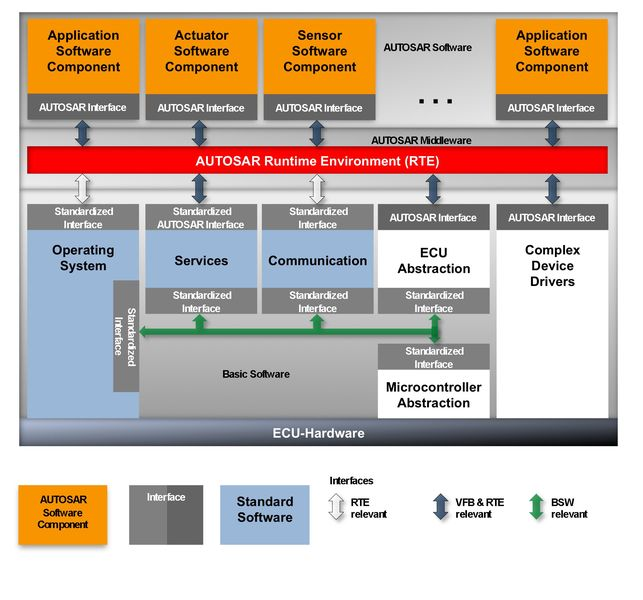
\includegraphics[width=.8\textwidth]{figure/layers_original.jpg}
%\caption{The layers of AUTOSAR architecture for an ECU (taken from~\cite{aa})}
%\label{fig:autosar}
%\end{figure*} 
%
However, %challenges also come with the popularity of AUTOSAR. As 
AUTOSAR just defines the architecture of the vehicle software system, while the implementation of the functionality is done by the manufacturers and suppliers themselves. Moreover, it is in general quite difficult to ensure that the quality expectations are met. %of which the quality is hard to ensure. 
This includes the %brings great challenges on the 
robustness of the developed AUTOSAR software components. %they developed. 
%AUTOSAR is mature, but such AUTOSAR software still needs to be improved. Researchers and developers are always willing to develop AUTOSAR software components with good robustness, they have been trying many different design ideas for development. 

In this paper we describe an industrial investigation made within Volvo AB in Gothenburg about using %made within 
Design by Contract as a means for improving the robustness of AUTOSAR software components. 
%looks like a promising %may be a good design 
%design idea for AUTOSAR software components. %As anticipated in Section~\ref{sec:background}, i
In Design by Contract, the relationship between a class and its clients is viewed as a formal agreement in which each party's right and obligations are described~\cite{jj}. In practice, it sets precise conditions to both the input and output of the components. %As the definition of robustness is ``the degree to which a system or component can function correctly in the presence of invalid inputs or stressful environmental conditions''~\cite{cc}. \
Since the output of one component is often the input of another component, this enables to check that the communication among components is correct. Design by Contract helps both checking the correctness of input and output of one software component, and %. Also, it checks 
the preservation of invariants inside the software component. %To achieve a high degree of robustness, Design by Contract is worth a try. The aim of this thesis is to answer the research question:
%
%\begin{itemize}
% \item \textbf{Is the use of Design by Contract a methodology to increase the robustness of AUTOSAR software components?}
%\end{itemize}


%The work in this thesis addresses this question. I apply 
The proposed approach is implemented and applied to the components of two AUTOSAR applications. %: Brake-Lighting and Brake-By-Wire (these two components are described in Section~\ref{sec:example}). 
%In line with the %With the design 
%idea of Design by Contract, conditions for input and output are set for the Brake-Pedal-Input-Handler component in the Brake-By-Wire system and the Brake-Light-Control component in the Brake-Lighting application. %As the Brake-Pedal-Input-Handler component is also used in the Brake-Lighting application, the connection of these two components is also considered and implemented. 
The output of our approach is a set of components enhanced with contracts. These  components %which are modified with input and output checking, 
are then tested by black-box testing with ARUnit testing tool. By comparing the test results of the original and modified components, we can conclude saying that Design by Contract greatly increases the robustness of AUTOSAR software components. In the paper we also identify and discuss limitations and weaknesses of the proposed approach.

The paper is structured as follows: Section~\ref{sec:background} provides background information that is needed to understand the approach. Section~\ref{sec:approach} presents the approach and Section~\ref{sec:implementation} describes its implementation. The validation of the approach is discussed in Section~\ref{sec:evaluation}. Related works are discussed in Section~\ref{sec:relatedWorks}. The paper concludes with final remarks and future research directions in Section~\ref{sec:conclusions}.


%the answer to the research question can be gotten.
\section{Background}\label{sec:background}



\subsection{AUTOSAR}
%AUTOSAR (AUTomotive Open System ARchitecture) \cite{aa} is a collaborative project initiated by several large manufactures and suppliers in automotive industry to establish a shared standard for automotive E/E architectures. It is driven by the intention of getting better flexibility, scalability, reliability, and quality when the complexity of E/E system is greatly increasing. This kind of increased complexity is mainly concerned with the growth of the functional scope. Besides the goal of making the developers concentrate on the realization of the functionality rather than the design of the architectures, the standard of AUTOSAR also makes components developed by different manufacturers or software companies be able to be integrated with well-defined interfaces. 

%\subsubsection{AUTOSAR Abstraction}
AUTOSAR is a standard architecture to make vehicle software applications independent of the hardware. 
AUTOSAR also makes components developed by different manufacturers or software companies able to be integrated through well-defined interfaces.
Every AUTOSAR application is distributed to one or more Electronic Control Units (ECUs). 
An AUTOSAR software component is defined as the encapsulation of part of the functionality of the AUTOSAR application~\cite{aa}. An AUTOSAR application is composed of one or several SW-Cs. How to describe the interfaces of these AUTOSAR SW-Cs is defined and standardized within AUTOSAR. Each component can only be distributed to one AUTOSAR ECU. This is the reason why the AUTOSAR SW-C is called as ``Atomic Software Component"~\cite{aa}. AUTOSAR does not prescribe the size of the SW-Cs and how the SW-Cs are implemented. But in order to be able to  integrate several AUTOSAR SW-Cs correctly, one formal and complete description for one SW-C is needed when it is implemented. The description introduces how to configure the infrastructure for the component when building the system. 

Communication between AUTOSAR software components are conducted by well-defined ports. A port is  defined by an AUTOSAR interface. It can either be a {\em Provided Port} which provides data or a {\em Required Port} which receives data. There are two main types of communication patterns supported by AUTOSAR. One is {\em Client-Server} and another one is {\em Sender-Receiver}. In the {\em Client-Server} pattern, the client sends a request for service, the server performs the requested service, %after receiving it 
and then responds to the request. An AUTOSAR software component (SW-C) can be both a client and a server. The {\em Sender-Receiver} pattern realizes asynchronous communication. %A sender sends information to one or several receivers without receiving back an answer. 
The time and way to send back information are decided by the receivers.

Communication between different ECUs is performed with a shared virtual bus, which consists of hardware interfaces provided by the basic software in AUTOSAR infrastructure. The Runtime Environment (RTE) is an implementation of the Virtual Functional Bus (VFB). It provides a uniform environment for communication between components~\cite{aa}. In this way, when moving a component to another ECU, developers do not need to change any code of the component. %The layered architecture of the AUTOSAR software for an ECU is shown in Figure~\ref{fig:autosar}. 



This work focuses on the application layer which consists of application software components. %Examples of components in AUTOSAR applications are given. 
%However, in the following we provide a short description also of the other layers to enable a better understanding of how the system works. %  for better understanding of how the system runs, short descriptions of related concepts of others layers are also given.


%\subsubsection{AUTOSAR Software Component}
%AUTOSAR software component is defined as the encapsulation of part of the functionality of the AUTOSAR application~\cite{aa}. An AUTOSAR application is composed of one or several SW-Cs. How to describe the interfaces of these AUTOSAR SW-Cs is defined and standardized within AUTOSAR. Each component can only be distributed to one AUTOSAR ECU. This is the reason why the AUTOSAR SW-C is called as ``Atomic Software Component"~\cite{aa}. AUTOSAR does not prescribe the size of the SW-Cs and how the SW-Cs are implemented. But in order to be able to  integrate several AUTOSAR SW-Cs correctly, one formal and complete description for one SW-C is needed when it is implemented. The description introduces how to configure the infrastructure for the component when building the system. The introductions to the components that I work on are given below. 
%
%\noindent {\bf Brake-By-Wire Application} - In this paper we make use of 
%In order to better understand the functionality of the selected AUTOSAR software components in this thesis, the software application that includes these components should be introduced. Here is the Brake-By-Wire application. 
%
%The Brake-By-Wire application is a research framework developed by the DEDICATE project~\cite{pp} that implements a brake-by-wire function distributed over five ECUs. It is not the real system that is used in the real trucks. It is proposed to give a example of distributed safety-critical system for validating research projects. The BBW application also includes an environment model of the vehicle in order to simulate the behaviour of the entire vehicle with regards to acceleration and braking~\cite{pp}. When using this application, the Brake Pedal ECU gets the signal of braking, does calculation and then sends a corresponding brake force request to each wheel.
%
%\paragraph{Brake-Pedal-Input-Handler Component}
%The distribution of the Brake-Pedal-Input-Handler component in the Brake-By-Wire system is shown in Figure~\ref{fig:BPIH}. The function of this component is to convert the hardware pedal input into a pedal position (0-100\%). The input of this component is an integer with 12 bits and the output is a percentage from 0\% to 100\%. It provides input for the Brake-Torque-Calculation component and the Brake-Light-Control component.
%
%
%\begin{figure}[htb]
%\centering
%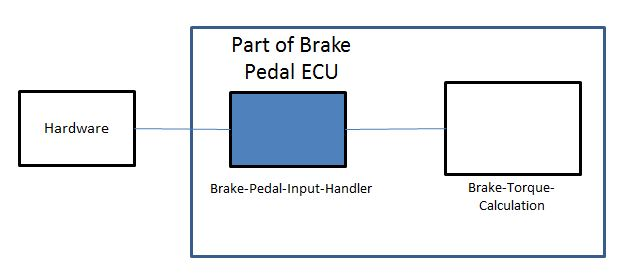
\includegraphics[width=\columnwidth]{figure/brakepedal1.jpg}
%\caption{Brake-Pedal-Input-Handler component distribution on ECU.}
%\label{fig:BPIH}
%\end{figure}
%
%\paragraph{Brake-Light-Control Component}
%
%The distribution of the SW-Cs in Brake-Lighting application is shown in Figure~\ref{fig:brakelighting}. The Brake-Light-Control Component is located on the BrakePedalECU. It inputs vehicle speed and brake pedal position (0-100\%) and outputs ON or OFF for the brake lights according to some rules. The basic rules~\cite{pp} are:
%
%\begin{enumerate}
%\item The brake light is always OFF when the pedal input is 0\%.
%\item The brake light is always fixed ON whenever the pedal input $>$ 0\% and the vehicle speed is $<$ 10km/h.
%\item From 10km/h and above the brake light will blink ON/OFF if emergency braking is active otherwise it is fixed ON.
%\end{enumerate}
%
%\begin{figure}[htb]
%\centering
%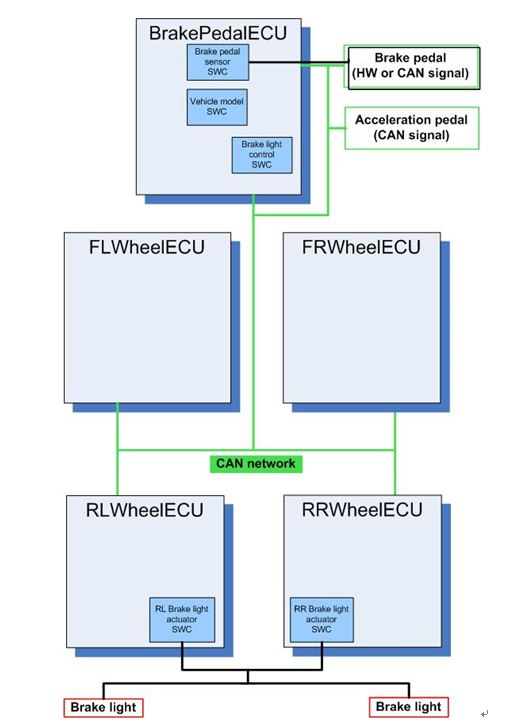
\includegraphics[width=.9\columnwidth]{figure/brakelighting.jpg}
%\caption{Brake lighting SW-Cs distribution on ECUs~\cite{pp}}
%\label{fig:brakelighting}
%\end{figure}

%
%\subsubsection{AUTOSAR Software Component Communication}
%Communication between AUTOSAR software components are conducted by well-defined ports. A port is  defined by an AUTOSAR interface. It can either be a Provider Port which provides data or a Required Port which requires data. There are two main types of communication patterns supported by AUTOSAR. One is Client-Server and another one is Sender-Receiver. In the Client-Server pattern, the client sends a request for service, the server performs the requested service, %after receiving it 
%and then responds to the request. An AUTOSAR software component (SW-C) can be both a client and a server. The Sender-Receiver pattern realizes asynchronous communication. A sender sends information to one or several receivers without receiving back an answer. The time and way to use the received information are decided by the receivers.
%%without getting a response from the receivers. And also, 
%%the time and way to use the received information are decided by the receivers. 

%\subsubsection{Virtual Functional Bus (VFB)}
%%The virtual functional bus (VFB)
%It is defined as the abstraction of the AUTOSAR SW-C interconnections~\cite{aa} on the vehicle. It enables the components on different ECUs to communicate with each other independent of the hardware and of which ECUs they locate. 

%\subsubsection{Runtime Environment (RTE)}
%%The runtime environment (RTE) 
%It is an information exchange center for communication inside one ECU or between different ECUs. It is the implementation of the VFB on a specific ECU~\cite{aa}. It provides the same interface for the SW-Cs to the AUTOSAR infrastructure and hardware despite where the SW-Cs are located. As different components are used in different applications, the RTE will be tailored in order to use resources more efficiently when the RTE is generated by the RTE generation tool. Sometimes, the RTE is tailored according to the configuration. All these make differences on the generated RTE of different ECUs. 
%
%\subsubsection{AUTOSAR Infrastructure}
%%The AUTOSAR infrastructure 
%It is a collection of basic software, which mainly consists of services, communication, operating system, ECU abstraction, microcontroller abstraction, and device drivers~\cite{aa}. Its function is to provide platform services to SW-Cs.


\subsection{Design By Contract}
Design by Contract, also known as programming by contract, is an approach for designing software, by which software can get better robustness. The key concept is ``viewing the relationship between a class and its clients as a formal agreement, expressing each party's right and obligations" \cite{jj}. The agreements are similar to the contracts in business. These contracts set conditions for input and output of software components. The conditions have three types, pre-condition, post-condition and invariant. When a client component calls an operation on a server component, the client component needs to meet the pre-condition which is specific for that operation. For the return of that operation, the requirements of the post-condition need to be meet, which is an obligation for the server component. Invariant is a certain property that are met for both of the two components. In this way, different components of a software system can collaborate with each other with high robustness. 

When Design by Contract was pioneered by Bertrand Meyer in the late 1980's, it was firstly used in the design of the Eiffel programming language~\cite{ii}. Later, this design philosophy of software started to be popular in languages with native support or with third-party support. 

%The following code~\cite{ii7} is a simple example of how Design by Contract works in C++. It is a short form of a class which omits some code not relevant to the example.
%
%\begin{figure}[htb]
%\centering
%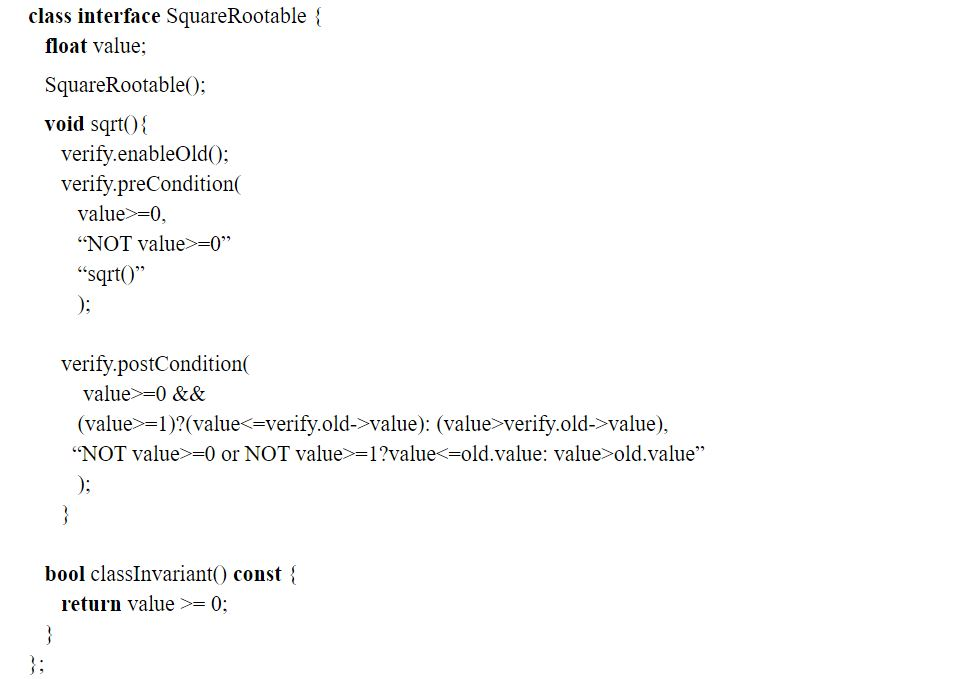
\includegraphics[width=0.9\linewidth]{figure/c++_code.jpg}
%\end{figure}
%
%This component functions as checking the input and output value of square root calculation. In this component, all the three types of conditions are set for the class. The pre-condition is that the input value should not be less than 0. The post-conditions are that the output value should be greater than 1 when the output value is less than the input value, and the output value should be greater than 0 and less than 1 when the output value is greater than the input value. The invariant for such a class is that the value should not be less than 0. If these criteria are not met, the calculation will not be conducted. This is a simple example for understanding such a design idea. 

In the C programming language, the application of Design by Contract is not obvious. % can be applied by assertions. 
For the reason that there are no classes in C, the subjects of the conditions are the functions. But the principles are similar. The caller function must meet all the preconditions of the callee function, and the callee function must meet its own post-conditions. The failure of either party of the contract is a bug in the software~\cite{jj}. Invariants in C are the conditions that must be hold for a structure or type\footnote{\url{http://www.onlamp.com/pub/a/onlamp/2004/10/28/design_by_contract_in_c.html}}. 

%When giving examples of setting conditions for software components in AUTOSAR, the conditions should derive from all the possible input (valid and invalid) and requirements specification. Using the Brake-Pedal-Input-Handler component as an example, the valid input is an integer from 0 to 4095 and the invalid input may be less than 0 or greater than 4095. The pre-condition can limit the input value in the valid range. Similarly, as the conversion calculation may make the output value less than 0\% or greater than 100\%. Obviously, the post-condition should check the output in the range of 0\%-100\%.

\subsection{Robustness}
Robustness is defined as ``the degree to which a system or component can function correctly in the presence of invalid inputs or stressful environmental conditions" in IEEE standard~\cite{cc}. The definition is similar to what is described in ISO 26262-1. The understanding of it is a bit different for software and hardware. For software, robustness is the ability to respond to abnormal inputs and conditions. For hardware, robustness is the ability to be immune to environmental stress and stable over the service life within design limits~\cite{bb}. 

In this paper we focus on the software part. Robustness of software refers to the capability of the %, on the one hand, good robustness means the 
system or component to %can 
(i) handle data correctly even when the input volume is very large, and (ii) %On the other hand, it should be able to 
handle invalid inputs to ensure the successful running of the system or component. As in the vehicle embedded system, most applications run repeatedly over a time period. The time period can be $5ms$, $10ms$ or $20ms$ according to the requirements of the application. %Considering the definition of Design by Contract, my work in this thesis mainly focuses on improving the capability of handling invalid inputs and ensuring valid outputs. That is how Design by Contract is applied.

The robustness of AUTOSAR software components is evaluated according to the rules described below:
\begin{itemize}
\item ARUnit (introduced in Section~\ref{sec:arunit}) is used to run black-box testing for the components. 
\item A list of data which may be valid or invalid is given as input to the component. 
\item For every input, the output can be data in the expected range, data outside the expected range, or error. 
\item Better robustness means more output data in the expected range, less output data outside the expected range and less errors. 
\item The comparison of them is used to benchmark the %shows the differences of different 
components' robustness.
\end{itemize}

 
\subsection{ARUnit}\label{sec:arunit}

ARUnit is a unit testing tool which provides a lightweight testing environment for AUTOSAR software components\footnote{\url{https://www.artop.org/arunit}}. It is based on Eclipse. After importing the components that need to be tested, it can compile the components and generate the run-time environment for each single AUTOSAR software component. %Of course, test cases can be defined in it as well for the reason that it provides an API to stimulate and query the state of the RTE from the outside. 
Test cases can be defined directly within the tool and moreover it provides an API to stimulate and query the state of the RTE from the outside. 
It is a quite convenient tool for operating unit testing effectively and efficiently. Figure~\ref{fig:ARUnit} shows how ARUnit generates RTE for AUTOSAR software components. %The way of how the data handled and exchanged inside  between component A and component B.

\begin{figure}[htb]
\centering
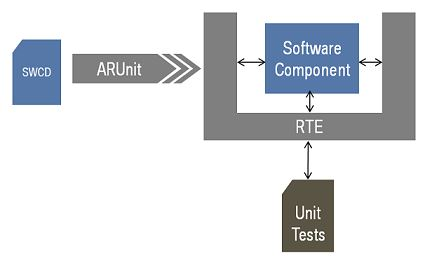
\includegraphics[width=0.9\linewidth]{figure/arunitin.jpg}
\caption{ARUnit provides RTE for single Software Component.}
\label{fig:ARUnit}
\end{figure}
\section{Design by Contract for AUTOSAR Software Components}\label{sec:approach}

%After studying several research methodologies and considering the context of this thesis, the research methodology described in~\cite{rr}, which is used for design research, is selected. The process of the research methodology for this thesis is described in Figure 1.1. The stages of the research methodology include problem identification, discussion \& suggestion, design \& development, evaluation, and conclusion \& report.
%
%In design research, the solution for solving one particular problem is investigated during the process of design and implementation \cite{rr}. In the context of this thesis, the problem is to verify if the use of Design by Contract is a methodology to increase the robustness of AUTOSAR software components. This problem also concerns how to implement software to apply Design by Contract to the components. In order to address the problem, different programming methods are proposed, discussed and implemented. After that, the AUTOSAR software components, which are enhanced with the programming method for Design by Contract, are tested with the unit test tool ARUnit. The robustness is evaluated from the results of the test. From the results, we can know whether Design by Contract helps improve robustness of AUTOSAR software components. The process and conclusion are documented and presented. 
%
%Besides some preparations for starting the thesis, the thesis 

This work has been realized in collaboration between the Chalmers University of Technology and Volvo AB. The work has been organized in three iterations, each of them including the following phases: (i) problem identification, (ii) discussion and suggestion, (iii) design and development, (iv) evaluation, and (v) conclusion and report. 
%work is done with 3 iterations. 
The first iteration was devoted to the investigation of \texttt{assert()} %was discussed and 
as the instrument to be used for applying the DbC approach to the original AUTOSAR SW-Cs. In the second iteration, we tried to set independent pre-condition components for every type of inputs. These two attempts were abandoned for their weaknesses as it is described in the following. Finally, in the third iteration we identified the method that we implemented and used. %The method builds new pre-condition, post-condition and invariant components. %presented in Chapter 4 was used and implemented. %Besides the iterations, I have weekly meeting with the supervisors at Chalmers and Volvo for delivering what has done, getting feedback and planning for next work. 

%In this chapter, three attempts of applying Design by Contract to AUTOSAR software components with different methods are described. The first and second attempts are abandoned for the problems and limitations they have. The final attempt which builds new pre-condition, post-condition and invariant components is adopted. The descriptions and figures are used to explain the solution in this chapter.

\subsection{First Iteration and Attempt}
%\subsubsection{Description}
Unfortunately the C programming language does not provide the language features that DbC needs. This first attempt focuses on the direct use of \texttt{assert()} to add input and output checks into the code. For example, there are two types of input and one type of output for one component. And the requirements for them are \texttt{input\_1 $>$ 0, input\_2 $<$ 0 and output $>$ 0}. Then we need to add \texttt{assert(input\_1 $>$ 0 \& input\_2 $<$0)} at the beginning of the code and \texttt{assert(output >  0)} at the end of the code. And also, if there are C-style structures or types in any places of the code, assertions are needed at these places as well. These assertions are used as the pre-conditions, post-conditions, and invariants for this component.

%\subsubsection{Problems \& Limitations}

\noindent {\bf Problems and Limitations:} A C-style assertion is not suitable for error handling especially in embedded software. In most situations, there are no screens available to show the information of the errors. What such software needs is an approach to detect and handle the errors. Moreover, there are many weaknesses of using assertions:

\begin{itemize}
\item Assertions lack robustness, there is a high intermix between application code and contracts, and there is a high code redundancy; 
\item The use of \texttt{assert()} requires to add extra code into the original component and this may also bring errors that might show up when running the preconditions, post-conditions and invariants checks;
\item Assert statements tend to intermix with application code and this is not good for readability, understandability, and reusability of the code;
\item Duplicate code is needed when invariants for a common structure or type exist in many different places in the code. 
\end{itemize}

Summarizing, \texttt{assert()} in C programming language does not make DbC reach desired effects to improve software components' robustness in AUTOSAR.

%First of all, assertions lack robustness, intermixing application code with contracts and code redundancy. Then, the use of \texttt{assert()} requires to add extra code into the original component and this may also bring errors that might show up when running the preconditions, post-conditions and invariants checks. Moreover, assert statements tend to intermix with application code and this is not good for readability, understandability, and reusability of the code. Finally, duplicate code is needed when invariants for a common structure or type exist in many different places in the code. Summarizing, \texttt{assert()} in C programming language does not make Design by Contract reach desired effects to improve software components' robustness in AUTOSAR.

\subsection{Second Iteration and Attempt}
%\subsubsection{Description}
As second attempt, we tried to set independent components for every type of input, output and structures in the original AUTOSAR software components. %Using the same example in Section 3.1.1, t
More precisely, there should be 3 components around the original component for every type of input, output and structures in the original component. In each of these components, there is a function which is used to check the value. %They are \texttt{function\_1(input\_1), function\_2(input\_2)} and \texttt{function\_3(output)}. 
These functions are invoked when needed by the original component. 

%\subsubsection{Problems \& Limitations}
\noindent {\bf Problems and Limitations:} 
This solution suffers of some limitations: 
\begin{itemize}
\item Typically, there is a huge number of types of input, output, and structures for one AUTOSAR software component. This will cause the creation of a large number of components and it will be hard to manage so many components;
\item In most conditions the requirements for one type of input, output or structure are not complex. It is not worth the effort of building so many new components just for one original component;
\item Other problems, such as redundancy of invoking these functions in the code of the original component and bad readability of the code, also exist.
\end{itemize}

Summarizing, this second solution is not exactly the best solution to improve software components' robustness in AUTOSAR.

%There are problems for this method. The most important one is that if there are a huge number of types of input, output and structures for one AUTOSAR software component, there will be the same number of components around the original component. It makes it hard to manage so many components. And also, in most conditions the requirements for one type of input, output or structure are not complex. It is not worth the effort building so many new components just for one original component. Other problems, such as redundancy of invoking these functions in the code of the original component and bad readability of the code, also exist.


\subsection{Third Iteration and Successful Attempt}
In this final attempt, we tried to build a pre-condition component, a post-condition component and an invariant component for one original component. The pre-condition component contains a function to check all the types of input. The post-condition component contains a function to check all the types of output. Also, the invariant component has functions to check all the structures or types in the original AUTOSAR software components. This method effectively limits the number of newly-built components and functions. It is also the method that we finally implemented and experimented. 

\begin{figure}[b]
\centering
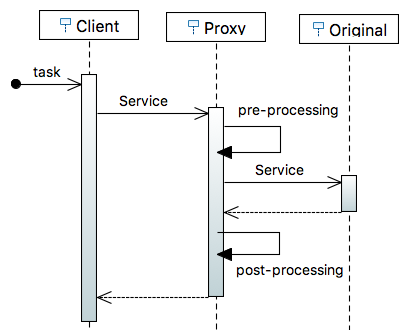
\includegraphics[width=.7\columnwidth]{figure/sequence1.png}
\caption{Process of how proxy pattern handles tasks}
\label{fig:proxyPattern}
\end{figure}


\subsubsection{Reference Patterns}
As mentioned in Section~\ref{sec:background}, the DbC approach considers the two sides of the contract as the caller and the callee (or the client and the server). For this reason, the traditional client-server pattern in the software architecture design is a very good reference pattern. In the client-server pattern, the component types are clients and servers, and the principal connector type for it is a data connector driven by a request/reply protocol used for invoking services~\cite{ii8}. A client is defined as a component that invokes services from a server component. A server is a component that provides services to clients. One component can be both a client and a server. This pattern is widely used as it ``factors out common services which are reusable"~\cite{ii8}. 

We got inspiration also from the Proxy patten for what concerns the 
%Another pattern that I drew lessons from is the Proxy patten. It is not how the components in this pattern distribute, but the way it handles
handling of the invoked service. %that is worthy of learning. 
As shown in Figure~\ref{fig:proxyPattern}, when a client component invokes a service from a server component, the proxy component will make pre-processing for the input and post-processing for the output. The pre-processing and post-processing can serve many purposes including converting formats. The idea is to exploit the pattern for input and output checking and to combine it with the widely approach.  %That is why I think it can also serve as input and output checking. This approach can combine with the Design by Contract approach. 


\subsubsection{Description of the Final Solution}
When combining the DbC approach with the two reference patterns, the most significant point is where to define the pre-conditions, post-conditions, and invariants. Figure~\ref{fig:solution} shows the design for the new components enhanced with DbC and how the components work together. The main processing component is almost the same as the original component. It is responsible for calculating or handling the input data and generating the output data. The newly-built pre-condition, post-condition and invariant components around it are responsible for data check. 

\begin{figure}[t]
\centering
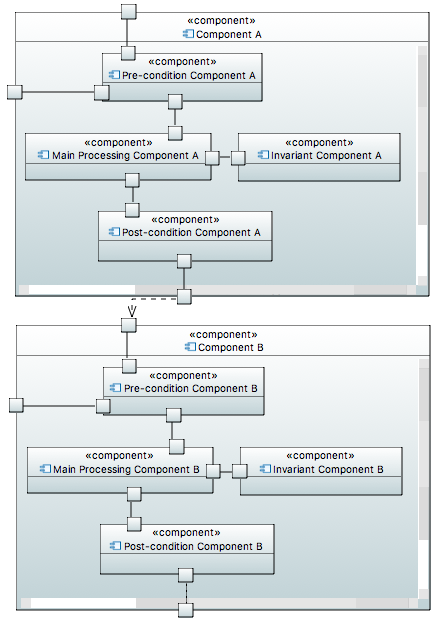
\includegraphics[width=.85\columnwidth]{figure/component11.png}
\caption{Design for AUTOSAR SW-Cs with Design by Contract}
\label{fig:solution}
\end{figure}

In the {\em Pre-condition component}, there is a function that works for checking all the input data. If the input is invalid or erroneous, it can be throw away or, if possible, it can be changed in %make it into 
a default and valid value. How to deal with it depends on the specific requirements. The {\em Pre-condition component} will then give the checked input data to the main processing component for further calculation. In the {\em Invariant component} one or more functions are defined. Each function is used for checking one structure or type in the code of the main processing component. When there is a structure or type in the code, it will invoke the corresponding function to check this structure before using it. In the {\em Post-condition component} there is a function that works for checking all the output data. It will make sure that the output is in the reasonable range. 

Considering how Proxy pattern handles input and output data, the newly-built pre-condition, post-condition and invariant components can be viewed as a proxy component. If one component needs the output data of another component as its input in an AUTOSAR software application, these two components can be seen as a client and a server. Figure~\ref{fig:dataExchange} shows how the input data are handled and exchanged between the components.

\begin{figure}[htb]
\centering
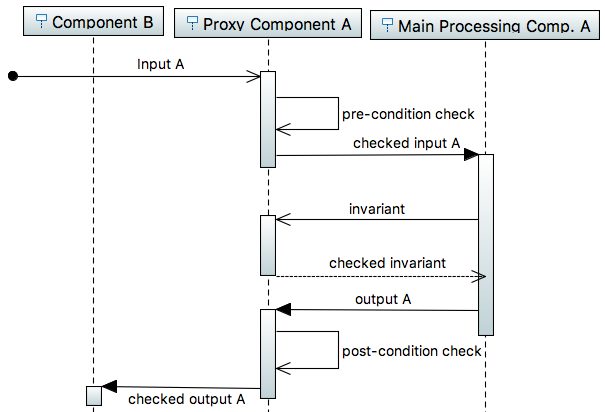
\includegraphics[width=\columnwidth]{figure/sequence2.png}
\caption{How data are handled and exchanged between components}
\label{fig:dataExchange}
\end{figure}

\section{Implementation}\label{sec:implementation}
This section introduces the process of setting up the development environment including exporting the Brake-Pedal-Input-Handler component and Brake-Light-Control component from the Arctic Studio, and importing them into ARUnit. Then, the implementation includes the identification of pre-conditions and post-conditions\footnote{In the considered components there was no need for invariant checks. As the functioning of the invariant component is similar to the functioning of the functions in the pre-condition and post-condition components, this will not affect the evaluation of our solution. In the AUTOSAR software components of other projects or applications, there are structures or types. Therefore invariant component can be used in those software components though it is not used here.}, and the design, modification and testing of the two software components. 

\subsection{Environment Setup and Components Import}
The PC used for the implementation and experimentation uses Windows 7 as the operating system and the two main development tools, Arctic Studio and ARUnit (introduced in Section~\ref{sec:background}), are installed correctly on it. Arctic Studio provides a complete embedded software development environment for automotive embedded software based on AUTOSAR\footnote{\url{http://www.arccore.com/products/arctic-studio}}. %Another development tool, ARUnit, has been introduced in Section~\ref{sec:background}.

Arctic Studio is the original development tool for the existing AUTOSAR SW-Cs. %The whole AUTOSAR software package that was developed in the DEDICATE framework project~\cite{pp} is in this tool. 
%\pat{More information on DEDICATE project} 
It makes the architecture easy to understand and the components easy to recognize and read. Driven by the industrial co-authors, and by reading through the code of the components and the available documentation, we selected the Brake-Pedal-Input-Handler Component and the Brake-Light-Control Component from the applications in this package as the components to be considered for the experiment. These two components are described in Section~\ref{sec:example}.

Arctic Studio and ARUnit are built for different purposes. ARUnit is more efficient for running and testing one single component or certain components. In order to modify and test the two selected components independently from the relevant components in the applications, the ECU, and the real running environment, we exported them from the whole package in Arctic Studio and imported them into ARUnit. The files that we imported into ARUint are the source files of the components and the software component description files of them. ARUnit is then used to generate the run-time environment for them. % according to these files when running them. 
Finally, code files used for testing are built in ARUnit as well. 

%In the software package of the DEDICATE framework project that the company gave me, I did not find a structure or type that should be checked with invariants in the components.\pat{cambia} That is why in the implementation part there are not descriptions about it. 
%As how the functions in the invariant component work is similar to the functions in the pre-condition and post-condition components, it will not affect the verification of this method. In the AUTOSAR software components of other projects or applications, there are structures or types. That means invariant component can be used in those software components though it is not used here.

\subsection{Selected AUTOSAR Software Components}\label{sec:example}
%An AUTOSAR software component is defined as the encapsulation of part of the functionality of the AUTOSAR application~\cite{aa}. An AUTOSAR application is composed of one or several SW-Cs. How to describe the interfaces of these AUTOSAR SW-Cs is defined and standardized within AUTOSAR. Each component can only be distributed to one AUTOSAR ECU. This is the reason why the AUTOSAR SW-C is called as ``Atomic Software Component"~\cite{aa}. AUTOSAR does not prescribe the size of the SW-Cs and how the SW-Cs are implemented. But in order to be able to  integrate several AUTOSAR SW-Cs correctly, one formal and complete description for one SW-C is needed when it is implemented. The description introduces how to configure the infrastructure for the component when building the system. %The introductions to the components that I work on are given below. 
In this section we describe the AUTOSAR software components we selected for the evaluation. These two components have been selected with the support of experts within Volvo AB and they are representative of the set of the existing AUTOSAR software components for the purpose of studying robustness. These components are used in many research projects within Volvo AB. 
%
%\subsubsection{Brake-By-Wire Application}
%In order t
To better understand the functionality of these components % selected AUTOSAR software components, %in this thesis, 
we first introduce the software application that includes them, i.e. the Brake-By-Wire application (BWB). %should be introduced. Here is the Brake-By-Wire application. 

The Brake-By-Wire is an application that is used in several research projects within Volvo AB. %is a research framework %developed by the DEDICATE project~\cite{pp} 
%that 
It implements a brake-by-wire function distributed over five ECUs. It is not the real system that is used in the real trucks. It is proposed to give an example of distributed safety-critical system for validating research projects. The BBW application also includes an environment model of the vehicle in order to simulate the behaviour of the entire vehicle for what concerns acceleration and braking~\cite{pp}. When using this application, the Brake Pedal ECU gets the signal of braking, does the calculation and then sends a corresponding brake force request to each wheel.

\subsubsection{Brake-Pedal-Input-Handler component}
The distribution of the Brake-Pedal-Input-Handler component in the Brake-By-Wire system is shown in Figure~\ref{fig:BPIH}. The function of this component is to convert the hardware pedal input into a pedal position (0-100\%). The input of this component is an integer with 12 bits and the output is a percentage from 0\% to 100\%. It provides input for the Brake-Torque-Calculation component and the Brake-Light-Control component.


\begin{figure}[htb]
\centering
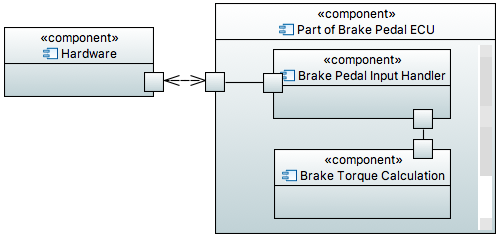
\includegraphics[width=.96\columnwidth]{figure/brakepedal1.png}
\caption{Brake-Pedal-Input-Handler component distribution on ECU.}
\label{fig:BPIH}
\end{figure}

\subsubsection{Brake-Light-Control component}

The distribution of the SW-Cs in the Brake-Lighting application is shown in Figure~\ref{fig:brakelighting}. The Brake-Light-Control component is located on the BrakePedalECU. It inputs vehicle speed and brake pedal position (0-100\%) and outputs ON or OFF for the brake lights according to some rules. The basic rules~\cite{pp} are:

\begin{enumerate}
\item The brake light is always OFF when the pedal input is 0\%.
\item The brake light is always fixed ON whenever the pedal input $>$ 0\% and the vehicle speed is $<$ 10km/h.
\item From 10km/h and above the brake light will blink ON/OFF if emergency braking is active otherwise it is fixed ON.
\end{enumerate}

\begin{figure}[htb]
\centering
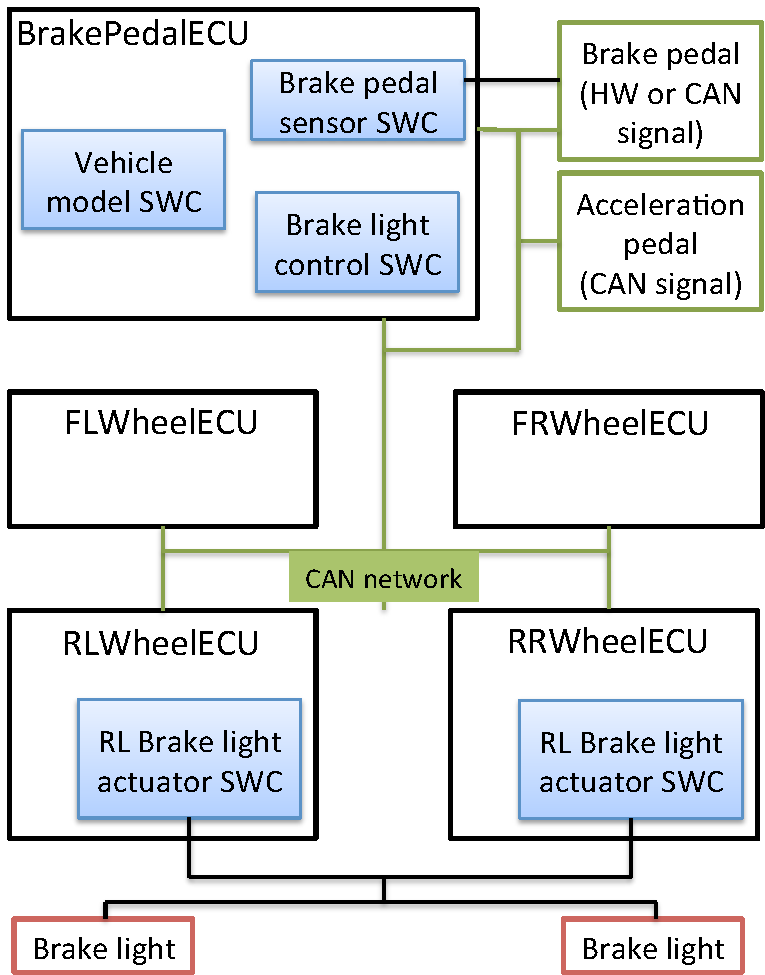
\includegraphics[width=.68\columnwidth]{figure/brakelighting.pdf}
\caption{Brake lighting SW-Cs distribution on ECUs~\cite{pp}}
\label{fig:brakelighting}
\end{figure}

\subsection{Process of Modifying the Brake-Pedal-Input-Handler Component}

In this section, we describe the analysis of the original component, the process of design, the modification and testing of the Brake-Pedal-Input-Handler component according to the Design by Contract approach.

\subsubsection{Issues of the Current Component}
Several issues were raised when reviewing the original component that may threaten the realization of the expected functionality and the robustness of the whole component. One issue is that there are no complete input checks for the component. %Inside t
The component does not handle the input in all the possible ranges of values that are mentioned in the documentation. %DEDICATE framework description \cite{pp}. 
In other words, the input check is too simple to deal with all the possible conditions. 

Another issue is that there is no output check to ensure that the data gotten from the component is completely correct for the next component that uses the data. Although the calculation in this component is not complex, the errors cannot be completely avoided at runtime. That is why output check is necessary.

Finally, other issues concern the internal logic and the readability of the component code. In the original component, the simple and incomplete input checks are mixed with the code that is responsible for the calculation. This makes the code hard to read and understand for developers. This may also threaten the robustness when modifying the code. 

\subsubsection{Identification of Pre-conditions and Post-conditions}

According to the documentation %DEDICATE framework description \cite{pp} 
and the package of all the program code, the Brake-Pedal-Input-Handler component is used to convert the analogue input from the pedal into a pedal position which is from 0\% to 100\%. The pedal provides an analogue input with the range from 10\% to 90\% of supply voltage (5V direct current), which means the voltage is about from 0.5V to 4.5V. If the analogue input is 0-0.5V, it means that it is an open circuit or short to ground. If the analogue input is 4.5-5V, it means that the battery level is too low. %it is short to battery. 
Both of them are errors. For the reason that the AD (Analog-to-Digital) converter of the micro-controller has not been calibrated, this inaccuracy has to be considered when building the software. % \cite{pp}. 
The output from the AD converter is the input for the software component we considered. The input is a 12 bit value, which uses 0 to represent 0V and uses 4095 to represent 5V. Of course, if considering that the input values of the test cases for this component can come also from the ARUnit, the input can possibly be less than 0 or greater than 4095. Thus, input values in these ranges are seen as invalid.

\begin{table}[htb]
\centering
\begin{tabular}{|c|c|c|c|c|c|c|c|}\hline
Range of Input Value\\ \hline
value $<$ 0\\ \hline
0 $<=$ value $<=$ 400\\ \hline
401 $<=$ value $<=$ 499\\ \hline
500 $<=$ value $<=$ 3500\\ \hline
3501 $<=$ value $<=$ 3700\\ \hline
3701 $<=$ value $<=$ 4095\\ \hline
value $>$ 4095\\ \hline
\end{tabular}
\caption{Ranges of input value}
\label{tab:BPIHRanegInput}
\vspace{-.4cm}
\end{table}

Table~\ref{tab:BPIHRanegInput} shows all the possible inputs of the Brake-Pedal-Input-Handler component. What we need to do next is to set contracts for the component. %That is to say, pre-conditions and post-conditions will be discussed in detail. 

When setting pre-condition part of the contracts, the information from requirements specification should be carefully considered to cover all the possible inputs. In this specific example the precondition considers as a valid input only an input value in the range 401 - 3700. 
%Here, pre-condition is that only the input value between 401 and 3700 is seen as valid and faultless. 
When the input value is less than 0 or greater than 4095, it is an invalid input. Input value in this range just appears in the testing environment in ARUnit\footnote{These values should not really come in real environments}. When the input value is in the range of  0-400 and 3701-4095, it is erroneous. Input values in this range represents 0-0.5V or 4.5-5V. They can be generated by the errors of hardware in the vehicles. For the post-condition, it should meet two requirements. Firstly, the output of the software component should be an integer from 0 to 100 to represent values from 0\% to 100\%. Then, the correctness check for the calculation within the component is needed. There are not structures or types used in this component. Hence, we do not need to set invariant checks for them.


\subsubsection{Design and Modification}

The aim of the modified software component is to solve the issues that exist in the original component with the Design by Contract approach. As mentioned in Section~\ref{sec:background}, the separation of the contracts and the component itself is a good practice. The architecture design of the new component is shown in Figure~\ref{fig:BrakePedalComponent}. 

\begin{figure}[htb]
\centering
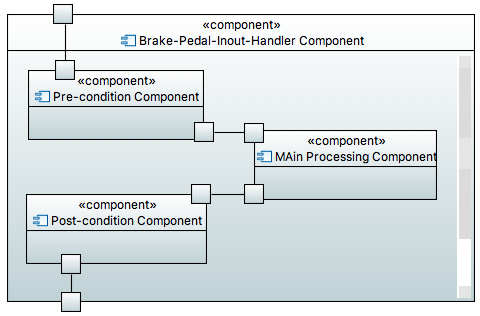
\includegraphics[width=.8\columnwidth]{figure/component222.png}
\caption{Design for the Brake-Pedal-Input-Handler Component.}
\label{fig:BrakePedalComponent}
\end{figure}

In the pre-condition component, there is a function that gets the pedal signal as input and verifies it for the main processing component. Only the valid and faultless data, which are greater than 401 and less than 3700, can enter into the main processing component. The invalid and erroneous data are detected and handled. 
In order to see the testing results intuitively, in our design it directly shows in the console of ARUnit that it is invalid or erroneous. For example, if the input is -100, the console shows it is an invalid input.  But when running in the real ECU, other approaches should be used to handle an invalid or erroneous input because of lack of a screen. The possible approaches may be the correction of the data or getting the next input data after some time. The main processing component works for calculation of the data and giving the results to the post-condition component for checks. The code for data processing in the main processing component is the same of the original component. In the post-condition component, a function used for checking the calculation results of the main processing component is defined. It checks if the calculation is correct and the output is in the range of 0\%-100\%. 

\subsubsection{Test}
In order to get to know if the modified component improves the robustness of the component, a testing program is created for the original component and the modified component in ARUnit. When running the testing program, the input data are sent into the component and the output data are shown on the console in ARUnit through the testing program. For better readability of the output data, some additional comments are attached with the output data to show the status of the calculation. Of course, this is used just in the testing environment to help developing the component and collecting information. In the real ECU, there are not such additional comments at runtime. 

In Table~\ref{tab:BPIHExpectedOutput}, some examples of input data in all possible ranges of the Brake-Pedal-Input-Handler Component are shown. According to the documentation, %DEDICATE framework description~\cite{pp}, 
the expected outputs of the software component are also included to help readers better understanding the testing. 

\begin{table}[htb]
\centering
\begin{tabular}{|c|c|c|}\hline
Range of Input Value & Input Example & Expected Output \\ \hline
value $<$ 0 & -100 & invalid input\\ \hline
0 $<=$ value $<=$ 400 & 200 & erroneous input\\ \hline
401 $<=$ value $<=$ 499 & 450 & 0, successful\\ \hline
500 $<=$ value $<=$ 3500 & 2100 & 53, successful\\ \hline
3501 $<=$ value $<=$ 3700 & 3600 & 100, successful\\ \hline
3701 $<=$ value $<=$ 4095 & 3900 & erroneous input\\ \hline
value $>$ 4095 & 6000 & invalid input\\ \hline
\end{tabular}
\caption{Examples of input for the Brake-Pedal-Input-Handler component and the expected output}
\label{tab:BPIHExpectedOutput}
\vspace{-.4cm}
\end{table}


In the testing period, 70 different input data are tested for both the original component and the modified component. If the output received from the component matches the expected output, we are in the case of a successful running. Referring to the Table~\ref{tab:BPIHExpectedOutput}, the tests that get valid output data such as 0, 53 and 100 are considered as successful tests that can be used by other components. Moreover, also 
%which can be used by other components are seen as successful tests, 
the tests that successfully detect invalid or erroneous inputs are seen as successful tests. The results of the testing are described in Section~\ref{sec:evaluation}. The robustness of the tested software component can be measured in terms of number or percentage of  %seen through how many of the
 test cases that are successful.

\subsection{Process of Modifying the Brake-Light-Control Component}

In this section, we describe the process of modifying the Brake-Light-Control component with the Design by Contract approach. This section emphasizes on the collaboration between the Brake-Light-Control component and the Brake-Pedal-Input-Handler component.

\subsubsection{Analysis and Identification of Pre-conditions and Post-conditions }

The existing issues for the Brake-Light-Control component are similar to the Brake-Pedal-Input-Handler component. It does not have complete input checks for the input data to cover all the possible input data. Some simple input data checks are mixed with the program code. Also, it lacks output checks. The modification for the original component is expected to solve these issues.

The Brake-Pedal-Input-Handler component is used to control the brake lights by the rules described in Section~\ref{sec:example}. Its input should be the pedal position and the vehicle speed. The pedal position is an output of the Brake-Pedal-Input-Handler component. The pedal position should be in the range 0\%-100\%. The range of the vehicle speed depends on different situations. Here, we set the highest vehicle speed as 300 km/h, which is obviously out of the range. Another factor that affects the output of the component is the status of emergency braking. The status of emergency braking can be active or inactive. In order to concentrate on the collaboration of the two modified components, the status of emergency braking is directly sent into the Brake-Light-Control component as another input without being included in the pre-condition. Thus, the pre-condition for this component is that the pedal position should be in the range 0\%-100\% and the vehicle speed should be in the range 0 km/h-300 km/h. For the post-condition, it should check if the calculation in the component is correct.

\subsubsection{Design and Modification}
 The design of the new Brake-Light-Control component is similar to the new Brake-Pedal-Input-Handler component. The pre-condition and post-condition are separated from the main processing component as the pre-condition component and the post-condition component. Figure~\ref{sec:testingEnvironment} shows how these components work together.

\begin{figure}[htb]
\centering
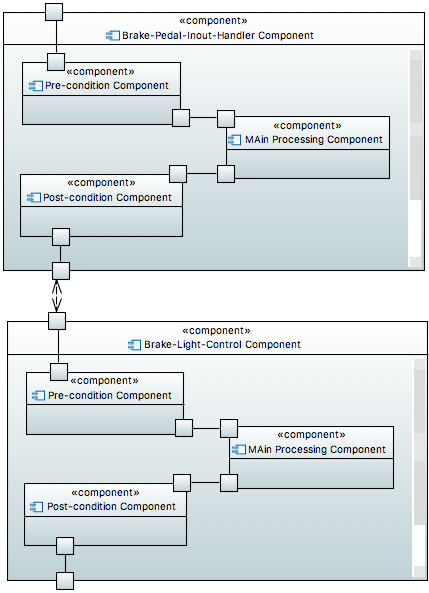
\includegraphics[width=0.9\linewidth]{figure/component33.png}
\caption{Design for the two selected components in the testing environment}
\label{sec:testingEnvironment}
\end{figure}


A function in the pre-condition component of the Brake-Light-Control component gets as input data from the Brake-Pedal-Input-Handler component and other sources, and then verifies the data for the main processing component. Only the input data with pedal position from 0\% to 100\% and vehicle speed from 0 km/h to 300 km/h are valid. The code for data processing in the main processing component is the same of the original component. In the post-condition component, a function used for checking the calculation results of the main processing component is defined. It checks if the status of braking light is correct.



\subsubsection{Test}
In order to know if the two modified components can collaborate with each other and improve the robustness, a testing program is created for the original components and for the modified components in ARUnit. When running the testing program, the input data are sent into both the two components. Data similar to those in Table~\ref{tab:BPIHRanegInput} are passed to the Brake-Pedal-Input-Handler component. Its output data are used as the input data for the Brake-Light-Control component with the vehicle speed and the emergency braking status. The output is the status of the brake lights. It can be ON/OFF/BLINK. Some comments are attached to the output to know which input is detected as invalid or erroneous. 

In Table~\ref{tab:inputData}, some examples of input data are shown. According to the documentation, the expected outputs of the software component are also included to help readers better understanding the testing. 

\begin{table}[htb]\footnotesize
\centering
\begin{tabular}{|p{1.5cm}|c|p{1.9cm}|p{1.9cm}|}\hline
Brake Pedal Input& Vehicle Speed & Emergency Braking Status & Expected Output \\ \hline
2000 & 5 & active & ON\\ \hline
450 & 35 & inactive & OFF\\ \hline
3000 & 35 & active & BLINK\\ \hline
200 & 35 & inactive & erroneous brake pedal input\\ \hline
500 & 400 & inactive & erroneous vehicle speed\\ \hline
\end{tabular}
\caption{Examples of input for the two selected components and the expected output}
\label{tab:inputData}
\vspace{-.4cm}
\end{table}


In the testing period, 30 different sets of input data are tested for both the original components and the modified components. If the output received from the components matches the expected output, it means that it is a successful testing. If it successfully detects the invalid or erroneous input, it is still seen as a successful testing. The results of the performed tests are described in Section~\ref{sec:resultsModified}. The robustness of the tested software component can be measured in terms of number and percentage of successful test cases.

%seen through how many of the test cases are successful.


\section{Evaluation}\label{sec:evaluation}

In the evaluation stage, black-box testing is performed with ARUnit test tool. The code of the software components is also in ARUnit, which is based on Eclipse. The steps of robustness evaluation are: %\\

\begin{enumerate}
 \item {Perform robustness testing in ARUnit of the original version of the software component.}
 \item {Input a list of valid and invalid data, and calculate the percentage of test cases that are successful. %output data is the result of successful running and also in the expected range. 
 This percentage is stored in the D1 variable.} %Keep this percentage as D1. }
 \item {In Eclipse, replace the original version of the software component with the software component which has been enhanced with Design by Contract.}
 \item {Input the same list of valid and invalid data of step 2, and calculate the percentage of test cases that are successful. %output data is the result of successful running and also in the expected range. 
  This percentage is stored in the D2 variable.} %what percent of the output data is the result of successful running and also in the expected range. Keep this percentage as D2.}
 \item {Compare D1 and D2. If D2 is greater than D1, it means the software component which is enhanced with Design by Contract has better robustness.}
\end{enumerate}

\subsection{Testing results of the Brake-Pedal-Input-Handler Component}

The testing results for the Brake-Pedal-Input-Handler component are shown in Table~\ref{tab:resultsTestingOriginalComp}. For the original component, it failed 15 times in the 70 test cases.  The modified component failed 0 time in the 70 test cases. The success rates of them are 78.6\% and 100.0\% respectively. Obviously, the modified component has better robustness and can handle more input data successfully. The analysis and evaluation are conducted in Section~\ref{sec:evaluations}.

\begin{table}[htb]
\centering
\begin{tabular}{|p{1.5cm}|c|c|c|}\hline
      & Successful Tests & Total Tests & Success Rates\\ \hline
Original Component & 55 & 70 & 78.6\% \\ \hline
Modified Component & 70 & 70 & 100.0\% \\ \hline
\end{tabular}
\caption{Results of tests for the Brake-Pedal-Input-Handler Component}
\label{tab:resultsTestingOriginalComp}
\vspace{-.6cm}
\end{table}

\subsection{Testing results of the Brake-Light-Control component}\label{sec:resultsModified}

The testing results for the Brake-Pedal-Input-Handler component %two modified components 
are shown in Table~\ref{tab:resultsTestingModifiedComp}. The original components failed 9 times in the 30 test cases.  The modified component failed 0 time in the 30 test cases. The success rates of them are 70\% and 100\%, respectively. Obviously, the modified component has better robustness and can handle more input data successfully.

\begin{table}[htb]
\centering
\begin{tabular}{|p{1.5cm}|c|c|c|}\hline
      & Successful Tests & Total Tests & Success Rates\\ \hline
Original Component & 21 & 30 & 70\% \\ \hline
Modified Component & 30 & 30 & 100\% \\ \hline
\end{tabular}
\caption{Results of tests for the two modified components}
\label{tab:resultsTestingModifiedComp}
\vspace{-.6cm}
\end{table}

\subsection{Evaluation}\label{sec:evaluations}

For the testing results, all input data of the failed test cases are in the ranges of invalid input or erroneous input. The reason of why getting such results is that the original components have incomplete and inaccurate input checks. They do not cover all the possible input data from different ranges. Although these invalid or erroneous input data seldom appear or will be replaced by the next input quickly in the real running in the ECU, they cannot be ignored. 

There are two main reasons that make the modified components get better results. The first one is that all possible input data have been considered by carefully analysing the documented specification when designing this new component. The invalid input data and erroneous input data have been handled in the pre-condition component and do not have the chance to get into the main processing component. The second reason is that the data from the main processing component are checked again in the post-condition component to ensure its correctness. The pre-condition and post-condition components are like two guards that check all the input and output data of the main processing component. 

The prerequisite of setting such pre-condition and post-condition components that can accurately cover all the possible input and output data, is that we need to have complete requirements for the components. 
According to experts within the company, %Some relevant information from the company can prove 
the two software components used in this work are representative for the entire set of the existing components for the purpose of studying robustness. It is important to highlight that, when developing AUTOSAR software components in the company, the bottom line for the requirements of the components is that the whole range of every input and output must be specified. And if they are not, someone will revise or update the requirements. It means that almost for every component the requirements specify the ranges of the input and output; this information can be used to help setting accurate pre-conditions and post-conditions for the components, similarly to what we have done in this paper.

For what concerns the design of the components, the components themselves and the collaboration among different components work well in the testing environment. For this design, there are clear and complete input and output checks that are conducted by the pre-condition and post-condition components. The main processing component can also focus on data processing. Moreover, the component code  becomes more readable and easier to modify when necessary. 

As already briefly discussed above, what is different from the real components in the ECUs is that in order to read the checking results more easily, the components in this work directly shows the results in the console. The way of detecting errors is the same. But in the real ECUs, if we detect errors, the component will use other ways to handle these invalid data. For example, in the Brake-Pedal-Input-Handler component, the component will switch to another sensor to get the input if the input from one sensor is invalid. In general the way of handling %How to handle the 
invalid data depends on the requirements. This is another reason why the well-specified requirements are important. 

%Some strengths and weaknesses of using Design by Contract in AUTOSAR software components have been mentioned in this thesis report more or less. 
Table~\ref{tab:strenghtsWeaknesses} shows a summary of strengths and weaknesses of using Design by Contract in AUTOSAR software components. 

\begin{table*}[htb]
\centering
\begin{tabular}{p{7.5cm} l p{9cm}}
\hline
\multicolumn{1}{c}{Strengths} & \multicolumn{2}{c}{Weaknesses  } \\
[.1ex]
\cline{1-1}  \cline{3-3} 
$\bullet$ Better robustness of the components and applications  &  & $\bullet$ Add more components which may also bring errors to the components \\
[.8ex]

$\bullet$ Increase readability and understandability of the code   &  & $\bullet$ Strict data checks may slow the components and applications down  \\
[.8ex]

$\bullet$ Convenient to refactor manually coded software components  &  & $\bullet$ Hard to modify the components of which the code is automatically  generated from some models \\
[-1.6ex]

$\bullet$ Low redundancy &  &          \\
%[1ex]

\hline
\end{tabular}
\caption{Strengths and weaknesses of the Design by Contract approach in AUTOSAR}
\label{tab:strenghtsWeaknesses}
\vspace{-.6cm}
\end{table*}


Another thing that needs to be evaluated here is in which situation the Design by Contract approach can be used to improve AUTOSAR software components' robustness. %As known from the DEDICATE framework description \cite{pp}, t
The code of some components is generated from TargetLink which is a modeling and development tool. Such kind of code is hard to read, import into ARUnit and modify manually. These components that have code automatically generated by TargetLink should follow a different approach. Contracts including pre-conditions and post-conditions should be embedded in code generation instead of trying to modify the code a-posteriori, as done by the approach proposed in this thesis. In the source base, nearly 50\% of the AUTOSAR software components are generated from TargetLink. Thus, at least 50\% of the components, i.e. those that have manually written code, can be easily enhanced with Design by Contract through the use of our approach. % to improve their robustness. 
As mentioned above our approach might be tuned so to be used in combination with code generation facilities. 
Finally, new AUTOSAR software components can certainly be designed and implemented with the Design by Contract approach.

For what concerns performance, for the two components we considered %for a few number of simpler and smaller components, 
performance is acceptable, also considering the gains in robustness. However, we should better investigate how deployment of DbC scales while considering various attributes/properties of components. We should also consider various aspects of performance, such as %Also, we can think of performance from various aspects. I actually suggested Yulai to consider various factors (
memory footprint, execution time, etc. and perform comparison between components without DbC and components with DbC. This is part of future work. %I am not sure if Yulai has performed such comparisons.

%\input{Discussion.tex}
\section{Related Works}\label{sec:relatedWorks}

Design by Contract (DbC) was firstly described by Bertrand Meyer~\cite{ii1} and included %in his several articles starting from 1986, which is introduced together with 
in his Eiffel programming language~\cite{ii}. %Later in 1992, in the article Applying Design by Contract
The work in~\cite{ii} shows that building software components on the basis of carefully designed contracts might reduce bugs and then improve 
%, Bertrand Meyer introduced the application of Design by Contract. In this article, he emphasized the significance of 
software reliability. %, which includes robustness and showed how to reduce bugs by building software components on the basis of carefully designed contracts. He defined the contract as the obligations and the benefits for the client and the supplier. Assertions, which include pre-conditions, post-conditions and invariants, were described by him to express contracts for software. 

In the last two decades DbC started to be popular in several programming languages, either through native support or with third-party solutions. 
The work in~\cite{Araujo2011} exploits DbC to concurrent programs. The authors extended the Java Modeling Language (JML) with constructs to specify  contracts %for Java programs 
and to %they present a runtime assertion checker 
%for 
verify assertions of concurrent Java programs. 
%We systematically evaluate the validity of system testing results obtained via runtime assertion checking using actual concurrent and functional faults on a highly concurrent industrial system from the telecommunications domain.
The same authors apply then the approach to a case study in %a highly concurrent industrial software system from 
the telecommunications domain to assess the effectiveness of contracts as test oracles in detecting and diagnosing functional faults in concurrent software~\cite{Araujo2014}. The authors conclude showing that DbC can be a valuable tool to improve the economics of software engineering.

%work in~\cite{Araujo2014} applies the approach
%Using Java as the target programming language, we tackle such challenges by augmenting the Java Modelling Language (JML) and modifying the JML compiler (jmlc) to generate runtime assertion checking code to support DbC in concurrent programs. We applied our solution in a carefully designed case study on a highly concurrent industrial software system from the telecommunications domain to assess the effectiveness of contracts as test oracles in detecting and diagnosing functional faults in concurrent software.

The work in~\cite{ii5} shows %presented 
how to specify the functionality of software components with the theory and methods of the Design by Contract approach. % in their paper in 2002. By their way of understanding Design by Contract, they concluded
The conclusion of the author is that the reliability and reusability of components can be enhanced by encapsulating operations 
%operations are encapsulated 
 within the components and by managing communications %are made 
 through the interfaces. %, it will make the components more reliable and reusable. 
 %Cheon et al.
 The work in~\cite{ii4} introduces an approach %a method in 2005, 
 to %model program variables to write and 
 check DbC assertions without referring to the program states; this makes the assertions more readable and maintainable.

%Benveniste et al.\cite{ii2} wrote one paper in 2011 about contract-based design which is similar to Design by Contract and its uses to address the challenges faced in designing large-scale complex embedded systems. Concepts and the key steps of contract-based design were introduced in this paper by giving three real examples.

%Th\"um et al.
The work in~\cite{ii3} introduced an approach for integrating DbC with feature-oriented programming. %; the idea is to define contracts for methods and their refinements to increase the reliability. Some case studies were also performed by them to gain and then share the insights.  

The work in~\cite{ContractsSystemsDesign} presents a methodology for contract-based system design. The authors identify also AUTOSAR software components as an interesting direction to be investigated. 
However, to the best of our knowledge, the use of DbC for AUTOSAR software components is not % the problem we tackle has not been
satisfactorily addressed in the literature. 
Our paper contributes exactly in this direction.

%The work of this thesis is based on the ideas and implementations from these related articles and work. As Design by Contract is used for objected-oriented languages in most situations and AUTOSAR SW-Cs are developed by C without any existing third-party tools that support Design by Contract, the author of this thesis needs to explore a new way for applying Design by Contract in AUTOSAR SW-Cs and evaluates the effect of improvement of robustness.
\section{Conclusions and future works}\label{sec:conclusions}

This work testifies that Design by Contract can be used for improving the robustness of AUTOSAR software components. % for better robustness.
Th approach we proposed in this work %My way in the thesis is 
proposes to build additional pre-condition, post-condition and invariant components around the main processing component. In other words, checks for input, output and invariant are separated from the original component. By testing the components modified in this way, the results prove that it improves robustness. This new design of components has strengths as better robustness, better readability, better understandability and low redundancy. It is very easy to apply this way to modify existing software components that are manually coded. % Two points are worth mentioning when applying this way. One is that the 
In order to apply the approach developers should analyse the documented specification or the stakeholders' requirements carefully to know all the possible values of the input, output and invariant. %Another is that the pre-condition, post-condition and invariant components should be well-defined to cover all the values known from the first point. Certainly, the weaknesses such as the possibility of the errors brought by additional components, also exist. That is why we need to go through careful consideration when applying this way of Design by Contract. The Design by Contract approach has been wildly used in many different software applications and tools supported by programming languages themselves or third-party tools. There may be other more effective ways of applying Design by Contract to AUTOSAR software components to improve robustness. That is worthy of further exploration.

%Many AUTOSAR software components are automatically generated from models in modeling tools. For example, some software components in the DEDICATE framework are modeled in Simulink or TargetLink and C source code is generated from TargetLink~\cite{pp}. These components are hard to modify with my way of applying Design by Contract. If the pre-condition, post-condition and invariant components can be modeled in the modeling tools and C source code can also be automatically generated, this will be a great progress.

%Further more, when searching for Design by Contract on the Internet, there are many third-party tools that can be used to support the programming languages that do not have Design by Contract language features. Developing 
%As future work we plan to %replicate the experiment within real
%apply the approach on real environments, i.e. on software components deployed on real trucks, and to make a large scale experiment. 
%it would be valuable to develop a tool that can support C language in AUTOSAR system to directly define pre-conditions, post-conditions and invariants for AUTOSAR software components. % is worth of trying.

%I believe that 
Concluding, DbC has high potential for industrial deployment, however, we need further investigations and evaluation results with more complex and real-life applications, e.g. by considering one complete feature such as cruise control. For example,  we need to better understand the impact that deploying DbC might have on real-time requirements, memory footprint, computational load,  etc. Such investigations will be part of our future work.

%Could be related to the previous comment. For a few number of simpler and smaller components, performance may not be a critical issue and could well be acceptable, considering the gains in robustness. However, we (at least, I) don't know how deployment of DbC scales with various attributes/properties of components. Also, we can think of performance from various aspects. I actually suggested Yulai to consider various factors (memory footprint, execution time, etc.) and perform comparison between component w/o DbC and component with DbC. I am not sure if Yulai has performed such comparisons.

%\section*{Acknowledgements}
%The work is partially supported by Software Center ({\small \url{http://www.software-center.se}}).			

\balance

\bibliographystyle{IEEEtran}
\bibliography{bibliography}

\end{document}